\documentclass[polish,twoside]{article}

% pakiet MwE
\usepackage{ze}

% tytul referatu
\title{Comments on the editing of articles for Zeszyty Energetyczny}
\shorttitle{Editorial notes...}
% tytul referatu w jez. angielskim
\titleEng{English title}
% Autorzy
\author{Jerzy Kulej\affmark[1], Dominik Bajoński\affmark[2]}
% Autorzy nagłówek
\authorheader{Jerzy Kulej}
% Afiliacje autorów
\affiliations{
    \affaddr[1]{Politechnika Kaliska, Katedra Procesów Cieplno-Przepływowych}
    \affaddr[2]{Wroclaw University of Science and Technology, Department of Energy Technologies, Turbines and Modeling of Heat-Flow Processes}
}
% Kontaktowy adres mailowy
\contactaddress{ze@pwr.edu.pl}

\begin{document}

\maketitle

\begin{ZEabstract}
Short description and comments on LaTeX paper formating.
\end{ZEabstract}

\begin{keywords}
\LaTeX, figures, equations
\end{keywords}

\normalsize

\section{Introduction}

Please prepare your paper according to the \textbf{KME-paper-template} and style ze.sty.
The \textbf{ze.sty} template file must be in the directory where paper (.tex) file is located. Preffered compilator is \textbf{PdfLatex}. A .pdf should be created without any errors. The source \emph{surname}.tex and the \emph{surname} .pdf version along with the drawings should be sent to the address \textbf{ze@pwr.edu.pl}.

The files with pictures should be called picture1, picture2, ... etc. in the order as they appear in the text of the article. Be sure to carefully check the article in .pdf format. Put the drawings in the * .jpg or * .png format. In the preamble, enter the title of your paper and your other details.

When compiling for the first time please do it twice so that the references to the literature are filled in. Provide literature items in accordance with the template. Try to follow the alphabetical order. Please quote using \textbf{$\ backslash$cite}\{Aref1\} which will create \cite{Aref1}. A simple manual for\ LaTeX will be posted on the \textbf{www.ze.pwr.edu.pl} page. Any other information will also be posted on this website. There are many tutorials, textbooks. Worth recommending is the readily available publication by Tobias Oetiker and others: \textit{Not too short introduction to \LaTeX}.

\section{Szczegółowe uwagi odnośnie redakcji artykułów}
Earlier work on the editing of our journal allowed us to create list of few important directions for authors:
\begin{enumerate}
    \item Please pay attention to the quality of the drawings included in the text. For the sake of readability, the font size in the drawings should be of the same size as the caption under the drawing. Avoid photos of test stands, photos documenting readings from instruments etc.
    \item Make sure that the end of the line does not end with a single letter. Blanks where lines must not be broken are marked in the source file by a tilde \~{}.
    \item  A single sentence closing paragraph cannot move to a new page. The text should be formatted in such a way as to choose the size of the figures and their location so as to make it possible to maintain the continuity of the thought expressed in the text. There is also the \textbf{newline} statement available. Please start a new paragraph with an indentation. If Latex did not do it automatically, it can be forced with the \indent instruction.
    \item Please write the chemical formulas as well as the dimensions of physical units in simple terms. Additionally please leave a space between the number and the physical unit, e.g. 1 m$^2$. 
    \item If a symbol is used in a mathematical formula and it is used in the text, it must be written in italics (italics).
    \item Paper should contain an even number of pages, not less than 8.. 
\end{enumerate}

\section{Examples of mathematical formulas}
An example of a text excerpt with \textbf{equations} is shown below.

The equations of motion of viscous and incompressible fluid have the form (equation \ref{eom} and \ref{incmp} - please write the reference to the equation as e.g. $\backslash$ref\{eom\}, and use $\backslash$label\{eom\} inside equation enviroment, which will form the reference base:
\begin{equation}\label{eom}
\frac{\partial{\mathbf{u}}}{\partial t}+(\mathbf{u} \cdot \nabla)\mathbf{u}=-\frac{1}{\rho}\nabla p+\nu \Delta \mathbf{u},
\end{equation}
\begin{equation}\label{incmp}
\nabla \cdot \mathbf{u}=0,
\end{equation}
where $\mathbf{u}=(u,v,w)$ velocity vector, $\rho$ -- density, $p$ -- pressure and $\nu$ -- kinematic coefficient of viscosity.

\section{Examples for figures and tables}

Examples of \textbf{charts, pictures and tables are presented below.}
A single graph or photo (Fig. \ref{image1} - reference to the image is created similarly to the example with the equation):
\begin{figure}[h!]
\centering
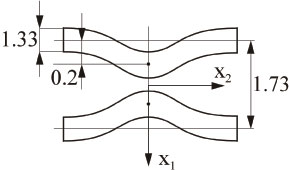
\includegraphics[width=0.3\linewidth]{figure1.jpg}
\caption{Jeden obrazek z podpisem}\label{image1}
\end{figure}

\noindent Two charts or photos side by side with two independent captions (Fig. \ref {image2} and Fig.~\ref{image3}):

\begin{figure}[htb]
\centering
\begin{minipage}[t]{0.42\linewidth}
\centering
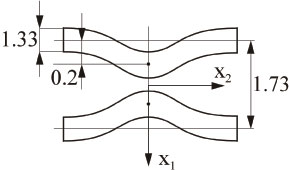
\includegraphics[width=0.65\linewidth]{figure1.jpg}
\caption{Two pictures side by side with two captions (left)}\label{image2}
\end{minipage}
\quad
\begin{minipage}[t]{0.42\linewidth}
\centering
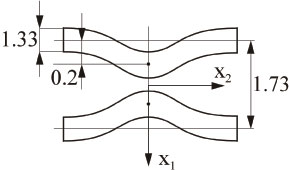
\includegraphics[width=0.65\linewidth]{figure1.jpg}
\caption{Two pictures side by side with two captions (right)}\label{image3}
\end{minipage}
\end{figure}

Below is an example of simple table created with table environment (Tab. \ref{tab1}. For fast creation of tables with larger datasets please use available online tools (for example this \href{https://www.tablesgenerator.com/}{Online table generator})

\begin{table}[!htb]
\caption{Przyspieszenie osiągane dla metody Jacobiego.}\label{tab1}
\centerline{
\begin{tabular}{|c|c|c|c|c|}
\hline
Liczba węzłów & tsl  &  tx &  nc & frm nc\\
\hline
32x32x32 & 4.05 & 6.61 & 6.94 & 12.32\\
64x64x64 & 17.71 & 26.32 & 31.26 & 52.82\\
128x128x128 & 24.78 & 29.95 & 43.67 & 58.89\\
\hline
\end{tabular}}
\end{table}

\noindent An additional example of creating a table.

\begin{table}[h]
    \centering
    \caption{Cryogenic coolers}
    \label{tab:cryocoolers}
    \begin{tabular}{@{}lll@{}}
    \toprule
    \begin{tabular}[c]{@{}c@{}}Cryooler\end{tabular} &
      \begin{tabular}[c]{@{}c@{}}Capacity range\end{tabular} &
      \multicolumn{1}{c}{ } \\ \midrule
    \begin{tabular}[c]{@{}c@{}}Turbo-Brayton\end{tabular}    & 18 - 250 kW at 120 K  \\
    \begin{tabular}[c]{@{}c@{}}Stirling\end{tabular}         & 2 - 8 kW at 120 K     \\
    \begin{tabular}[c]{@{}c@{}}Gifford-McMahon\end{tabular}  & 14 - 600 W at 80 K     \\
    \begin{tabular}[c]{@{}c@{}}Single-stage Pulse Tube\end{tabular}  & 12 - 90 W at 80 K  \\
    \begin{tabular}[c]{@{}c@{}}Miniature Pulse Tube\end{tabular}       & 3 - 10 W at 80 K    \\
    \begin{tabular}[c]{@{}c@{}}Joule-Thomson\end{tabular}       & 100 W at 120 K   \\ \bottomrule
    \end{tabular}
\end{table}

\section{Summary}

The purpose of a summary is to give the reader a clear, objective picture of the original text. Most importantly, the summary restates only the main points of a text.

\begin{thebibliography}{10}
{\small
\bibitem{Aref1} Aref H.  \textit{Motion of three vortices}, Phys. Fluids \textbf{22} (3), 393-400, 1997
\bibitem{Holden_etal_2007} Holden H., Karlsen K.H., Lie K.-A., Risebro W.H. \textit{Splitting Methods for Partial Differential Equations with Rough Solutions}, Society for Industrial and Applied Mathematics,  2007
\bibitem{LeVeque_2010} LeVeque R.J. \textit{Finite Difference Methods for Ordinary and Partial Differential Equations}, European Mathematical Society, 2010
\bibitem{Kudela_Kosior_2013} Kudela H., Kosior A. \textit{Parallel reconnection of vortex tube reconnection using a graphics card and the 3D Vortex-in-Cell method}, Procedia IUTAM, \textbf{7}, 59-66, 2013
}
\end{thebibliography}
\end{document}
